\documentclass[aspectratio=169,10pt]{beamer}

\usetheme{Madrid}
\setbeamertemplate{navigation symbols}{}
\setbeamertemplate{footline}[frame number]

\usepackage[T1]{fontenc}
\usepackage[utf8]{inputenc}
\usepackage{amsmath,amssymb}
\usepackage{graphicx}
\usepackage[ruled,vlined,linesnumbered]{algorithm2e}

\newcommand{\Dtot}{D_{\mathrm{tot}}}
\newcommand{\Dfar}{D'}
\newcommand{\Dloc}{D}
\newcommand{\rep}{\mathrm{rep}}
\newcommand{\KL}[2]{\mathrm{KL}\!\left(#1 \,\middle\|\, #2\right)}

\title{LongRange-PFN}
\subtitle{Recursive latent summaries beyond the context window}
\author{Gabriel Abad \\ FGV EMAp}
\date{}

\begin{document}

\begin{frame}
  \titlepage
\end{frame}

\begin{frame}{The Prior-Fitted Network paradigm}
  \[
    p(y \mid x, D)
    \;=\;
    \int p(y \mid x, \rho)\, p(\rho \mid D)\, d\rho
  \]
  \begin{itemize}
    \item \textbf{In context:} pretrain on a prior; at test time the dataset is the context and prediction is one forward pass.
    \item \textbf{Synthetic prior:} datasets \(\mathcal{D} \sim p(\mathcal{D})\). Minimizing NLL approximates the Bayesian predictive.
    \item \textbf{Bar distribution:} density over \(B\) buckets with fixed borders (here \(B=100\)).
  \end{itemize}
  \vspace{0.6em}
  \footnotesize TabPFN is the tabular instance of this paradigm. It inherits the same ceiling: the window seen in training.
\end{frame}

\begin{frame}{The window is both memory and ceiling}
  \begin{columns}[T]
    \begin{column}{0.48\textwidth}
      \begin{block}{Two costs}
        \[
          O(|\Dtot|^2)
        \]
        Quadratic attention, and a context size the model never practiced.
        Here, \(N=80\).
      \end{block}
      \begin{itemize}
        \item Subsampling drops likelihood terms and widens the posterior.
        \item Test-time selectors (kNN, MICP, CRUMB) keep real points, with no persistent state.
        \item TuneTables / ICD optimize per dataset; they do not amortize.
      \end{itemize}
    \end{column}
    \begin{column}{0.48\textwidth}
      \begin{alertblock}{What is missing}
        A fixed-size, amortized latent summary that keeps what \(\Dfar\)
        contributed to \(p(\rho \mid \cdot)\), and that can be updated in a stream.
      \end{alertblock}
      \footnotesize AutoCompressors are close in language modeling, but train next-token likelihood,
      not a Bayesian teacher's predictive.
    \end{column}
  \end{columns}
\end{frame}

\begin{frame}{LongRange-PFN at a glance}
  \begin{center}
    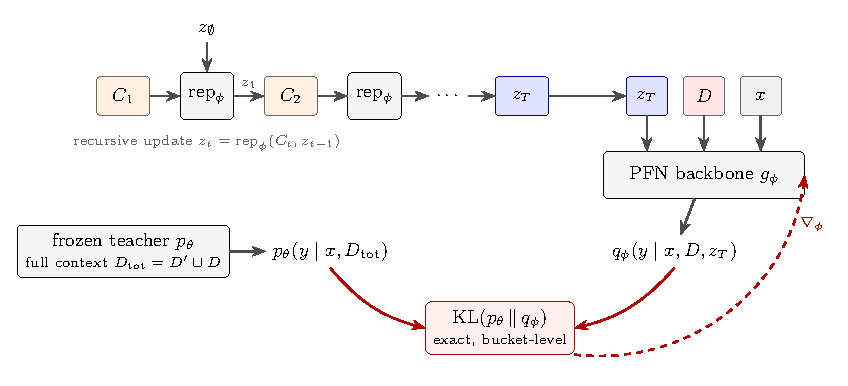
\includegraphics[width=0.95\textwidth]{assets/architecture_standalone.pdf}
  \end{center}
\end{frame}

\begin{frame}{Predictive KL distillation}
  \[
    \KL{p_\theta(y \mid x, \Dfar \cup \Dloc)}
        {q_\phi(y \mid x, \Dloc, \rep_\phi(\Dfar))}
  \]
  \begin{enumerate}
    \item Frozen teacher \(p_\theta\) sees full context; student \(q_\phi\) sees \(\Dloc\) plus summary \(z\).
    \item Shared bucket borders yield an exact categorical KL, with no sampling.
    \item Recursive update \(z_t = \rep_\phi(C_t, z_{t-1})\), with \(T \in \{1,2,3\}\) during training.
    \item Forward KL pushes errors toward over-coverage; \(z\) carries what \(\Dfar\) changes in \(p(\rho \mid \cdot)\).
  \end{enumerate}
\end{frame}

\begin{frame}{Algorithm 1: recursive KL distillation}
  \begin{algorithm}[H]
    \DontPrintSemicolon
    \KwIn{frozen teacher \(p_\theta\); prior \(p(\mathcal{D})\); window \(N\); bucket borders}
    initialize backbone of \(q_\phi\) from \(\theta\); summarizer encoders from \(\theta\)\;
    \For{each step}{
      sample \(\mathcal{D} \sim p(\mathcal{D})\) with \(N\) context and \(M\) query points\;
      sample \(|\Dloc|\) (or \(\Dfar = \emptyset\)); split \(\Dtot = \Dfar \cup \Dloc\); sample \(T \in \{1,2,3\}\)\;
      \(z \leftarrow z_\emptyset\)\;
      \For{\(t = 1, \dots, T\)}{
        \(z \leftarrow \rep_\phi(C_t, z)\)
      }
      \(\mathcal{L} \leftarrow \frac{1}{M}\sum_{x}
        \KL{p_\theta(y \mid x, \Dtot)}{q_\phi(y \mid x, \Dloc, z)}\)
        \tcp*{exact, bucket-level}
      update \(\phi\) by SGD on \(\mathcal{L}\)\;
    }
    \caption{Recursive KL distillation of LongRange-PFN}
  \end{algorithm}
\end{frame}

\begin{frame}{Proposition 1: information-flow certificate}
  Any predictor \(q\) that depends on the data only through \((x,\Dloc)\) satisfies
  \[
    \mathbb{E}\bigl[-\log q(y \mid x, \Dloc)\bigr]
    \;\ge\;
    \mathbb{E}\bigl[-\log p(y \mid x, \Dloc)\bigr].
  \]
  \begin{itemize}
    \item The gap is a KL (Gibbs). Under the GP prior the right-hand side is closed form.
    \item If the student's NLL falls below this bound, information from \(\Dfar\) reached the predictor,
          and it can only have arrived through \(z\).
  \end{itemize}
\end{frame}

\begin{frame}{Data and setup}
  \begin{columns}[T]
    \begin{column}{0.32\textwidth}
      \textbf{1D GP (RBF)}\\[0.3em]
      \footnotesize Lengthscale \(0.1\), noise \(10^{-2}\).
      Analytic posterior. From \(|\Dtot|=80\) to \(320\), the exact predictive improves by \(\approx 0.061\) nats.
    \end{column}
    \begin{column}{0.32\textwidth}
      \textbf{TabArena}\\[0.3em]
      \footnotesize Regression, OpenML study 457.
      Budget \(n=0.1N\). Targets z-scored on the training split.
    \end{column}
    \begin{column}{0.32\textwidth}
      \textbf{Selectors}\\[0.3em]
      \footnotesize Uniform, per-query kNN, MICP, CRUMB: all wrapped around the same frozen teacher.
      Shift along \(x\): \(\tau=0\) vs \(\tau=1\).
    \end{column}
  \end{columns}
  \vspace{1.2em}
  \footnotesize Teacher: 4 layers, \(e=128\), 0.9M, window 80.
  Student: 1.6M, 3-layer summarizer, \(k=16\).
\end{frame}

\begin{frame}{Closing the truncation gap}
  \begin{columns}[T]
    \begin{column}{0.38\textwidth}
      {\Large\bfseries 97\%}\\[0.3em]
      of the truncation gap recovered at \(|\Dloc|=10\).
      \vspace{0.8em}
      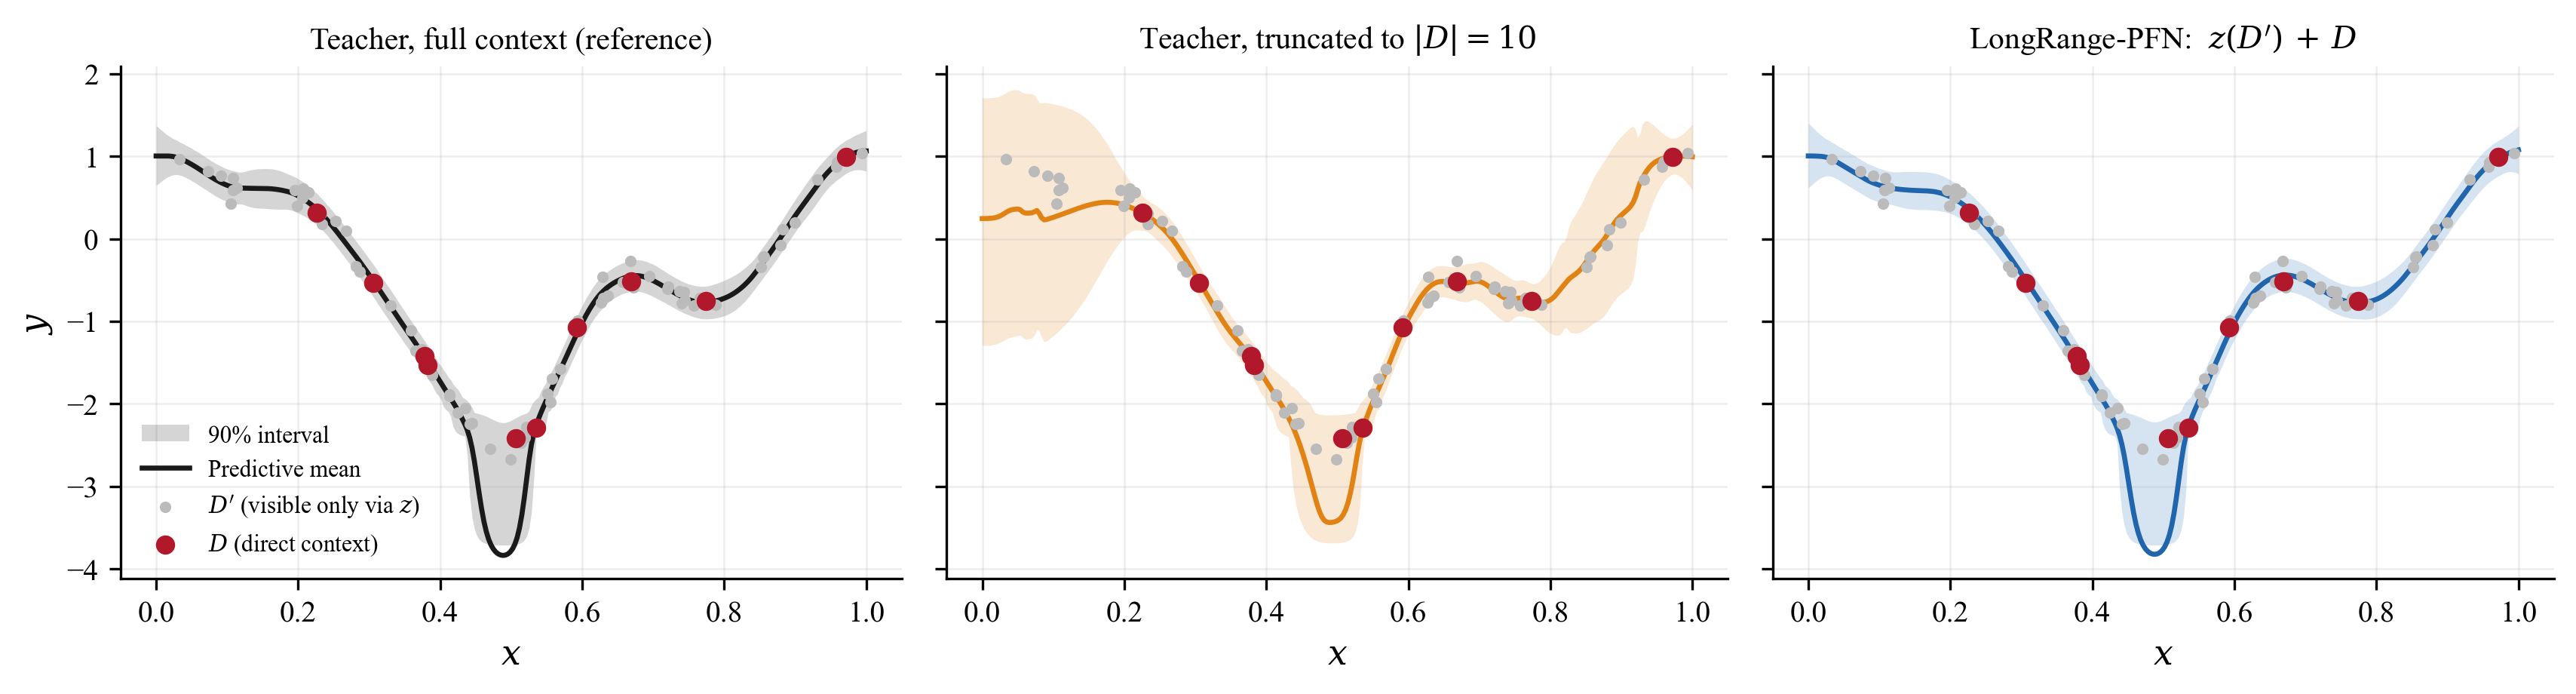
\includegraphics[width=\linewidth]{../results/qualitative.png}
    \end{column}
    \begin{column}{0.60\textwidth}
      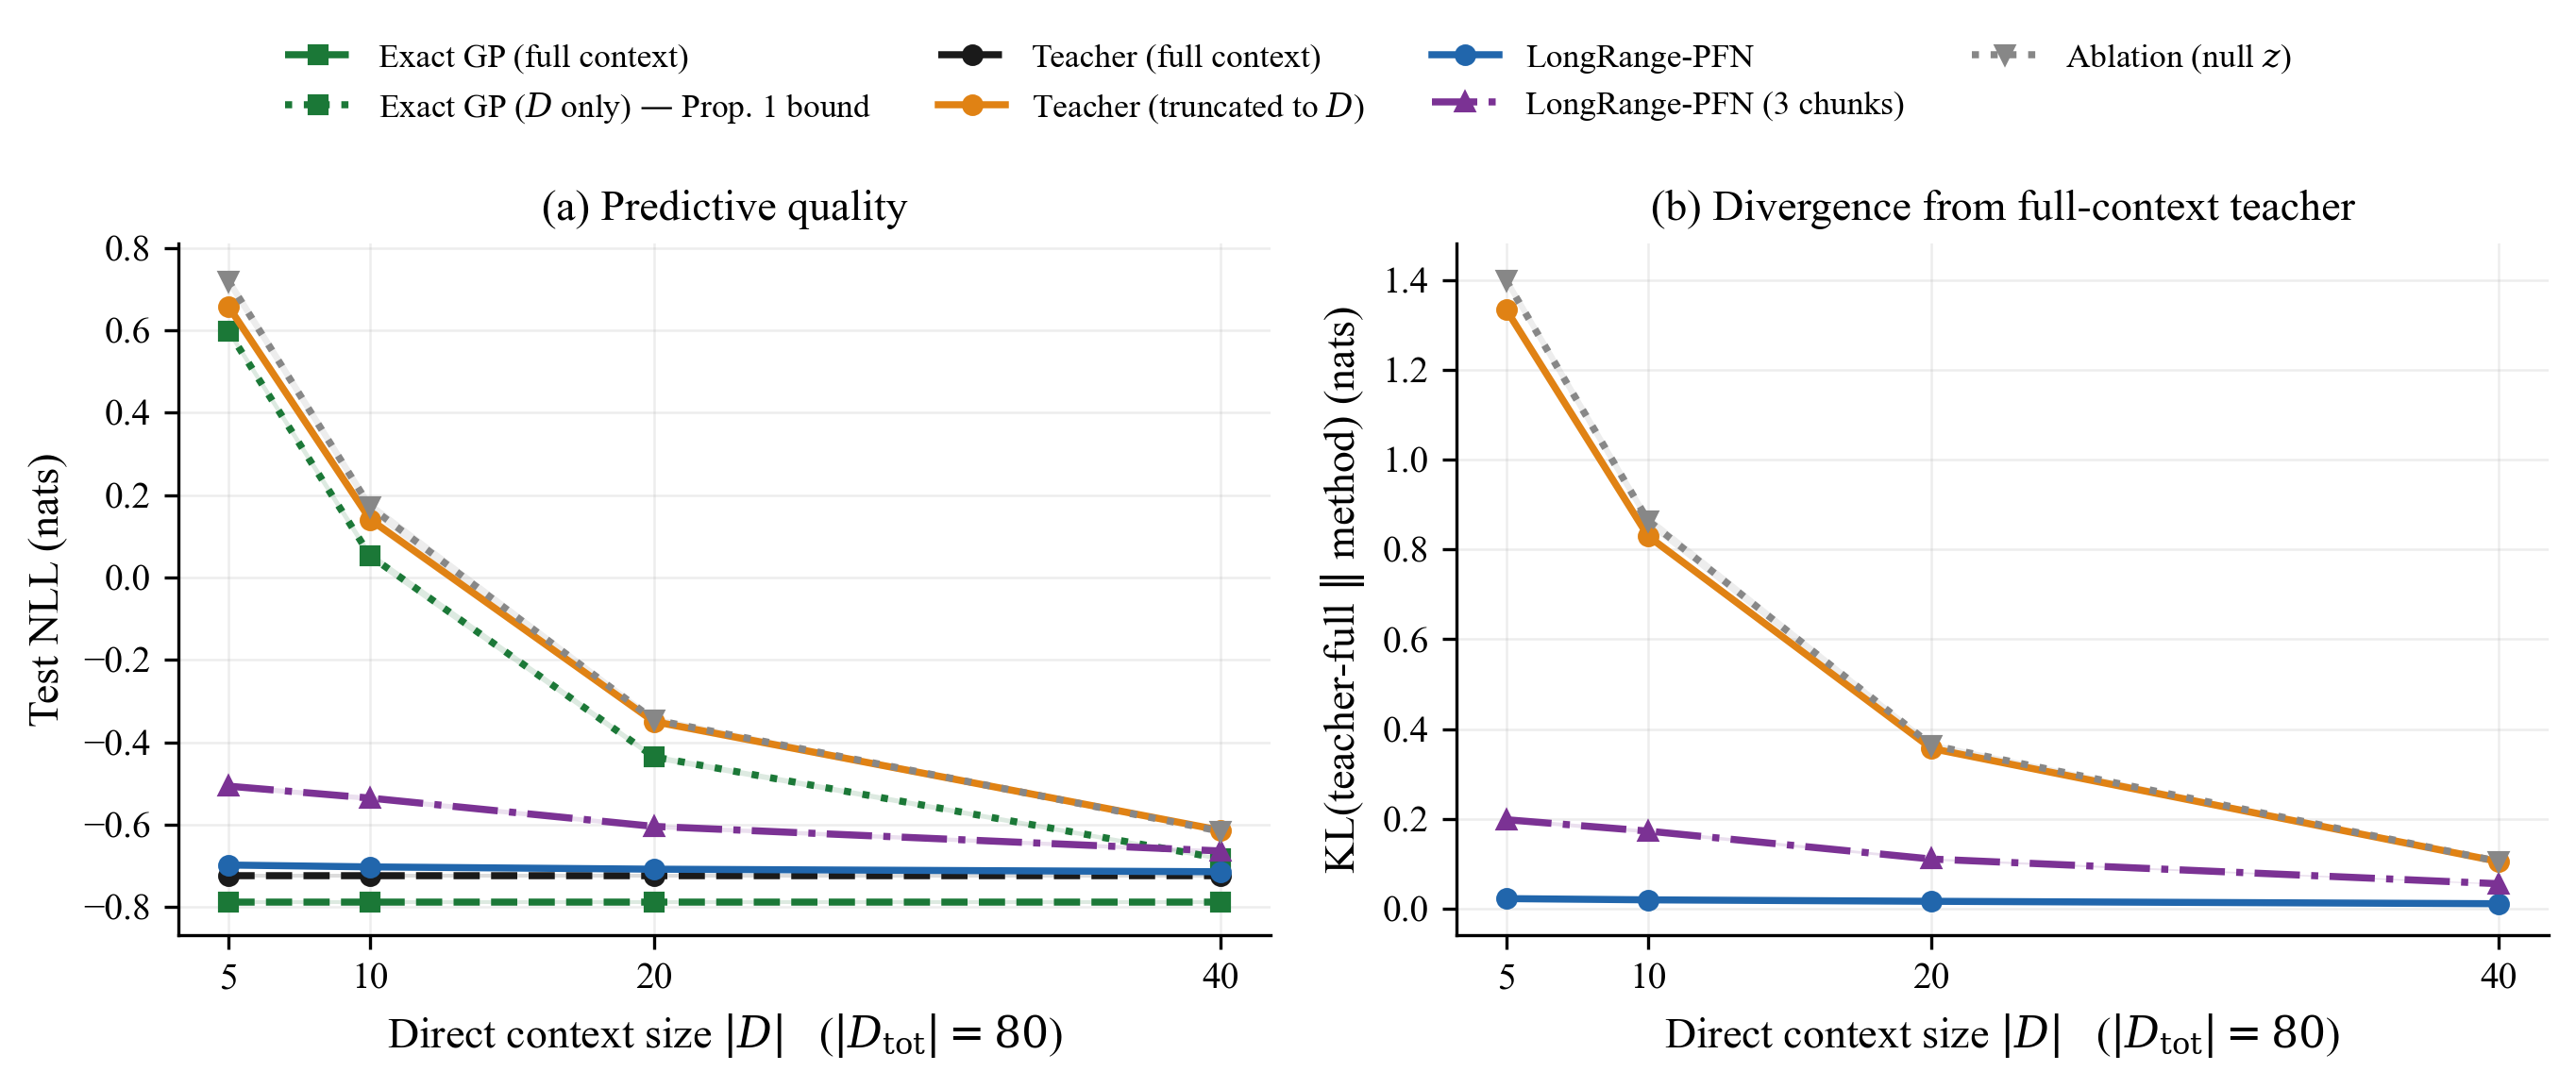
\includegraphics[width=\linewidth]{../results/sweep.png}
    \end{column}
  \end{columns}
\end{frame}

\begin{frame}{Streaming beyond the window}
  \begin{center}
    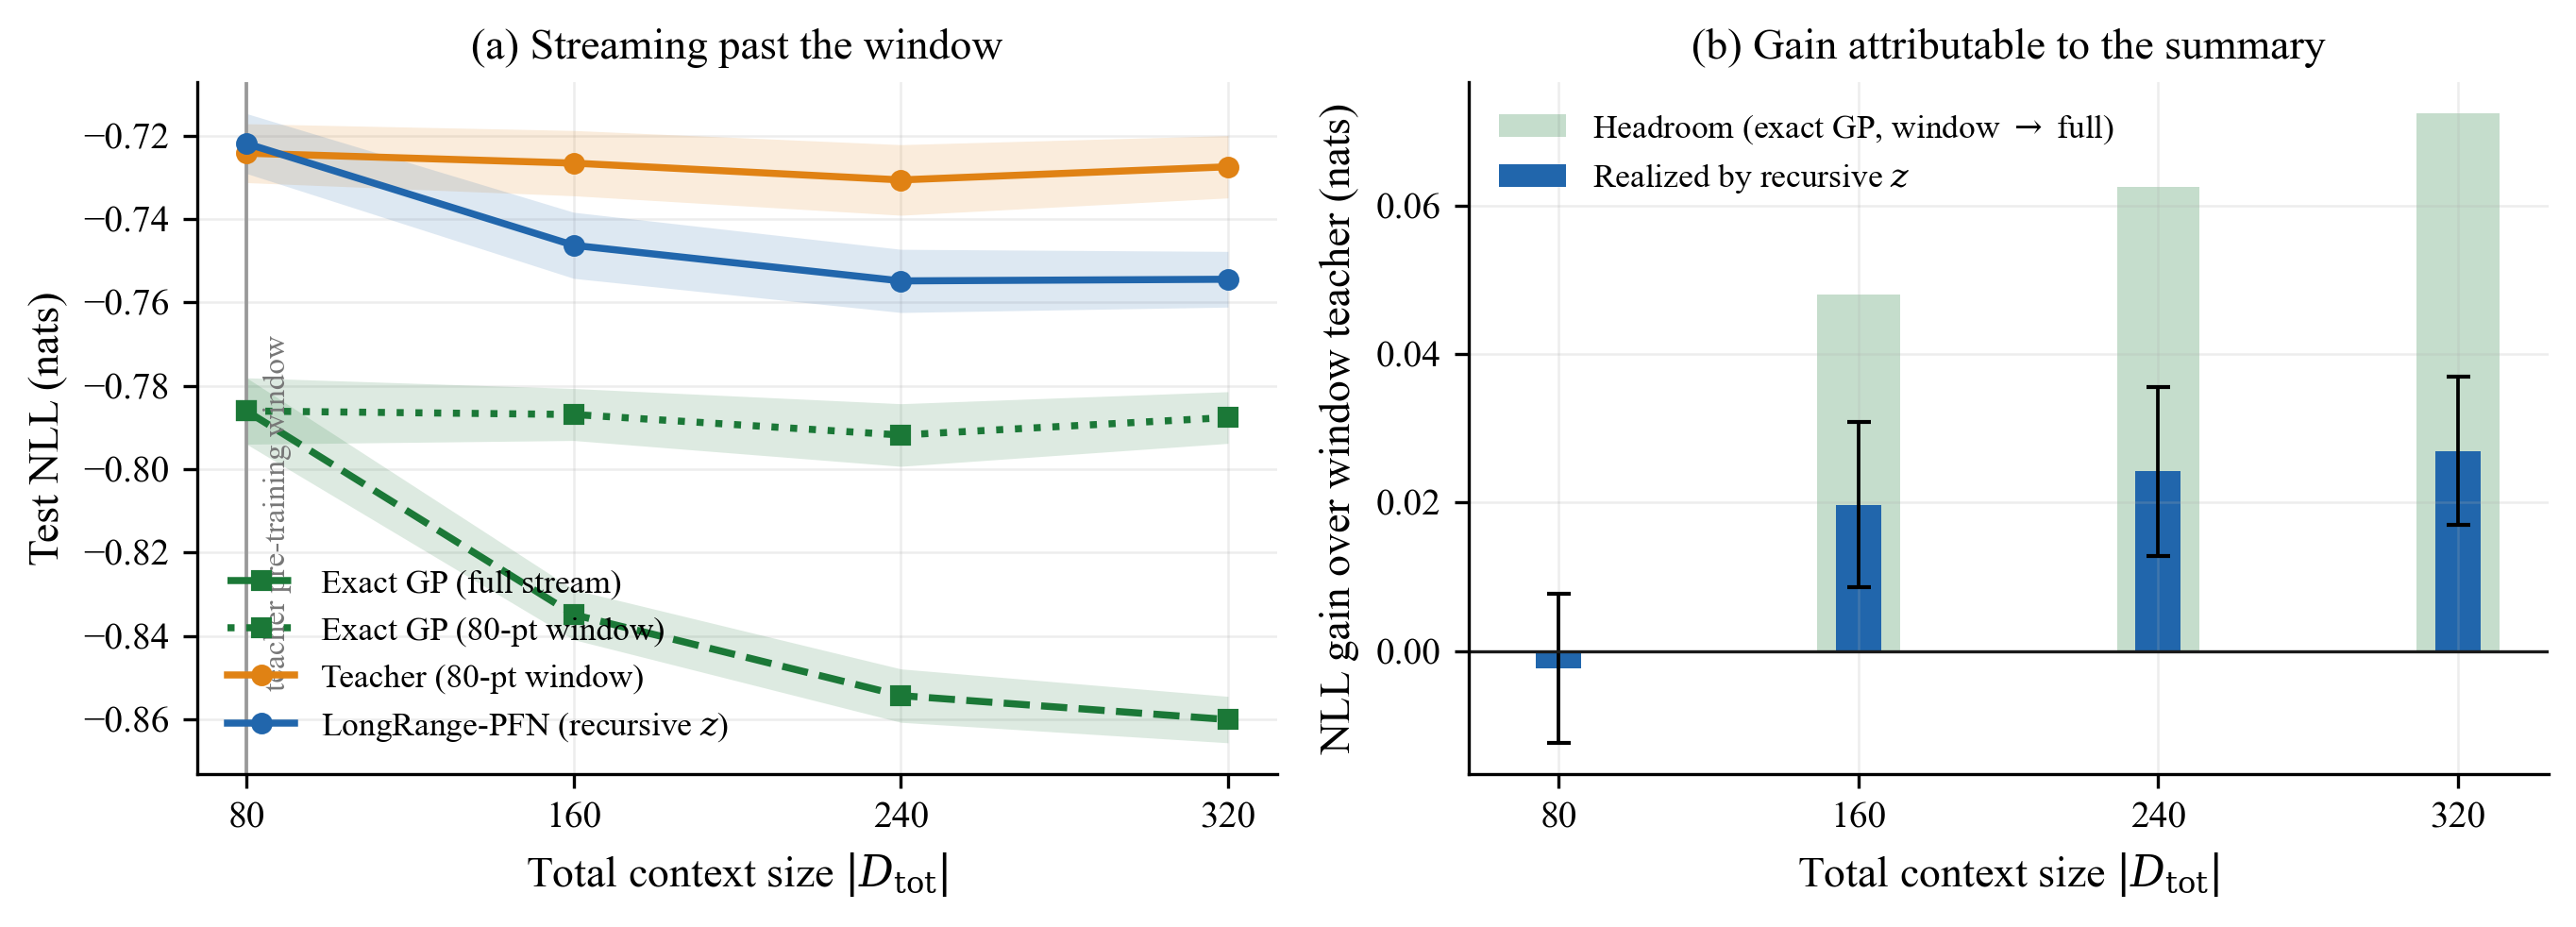
\includegraphics[width=0.95\textwidth]{../results/beyond_window.png}
  \end{center}
\end{frame}

\begin{frame}{When the summary wins, and when it loses}
  \begin{center}
    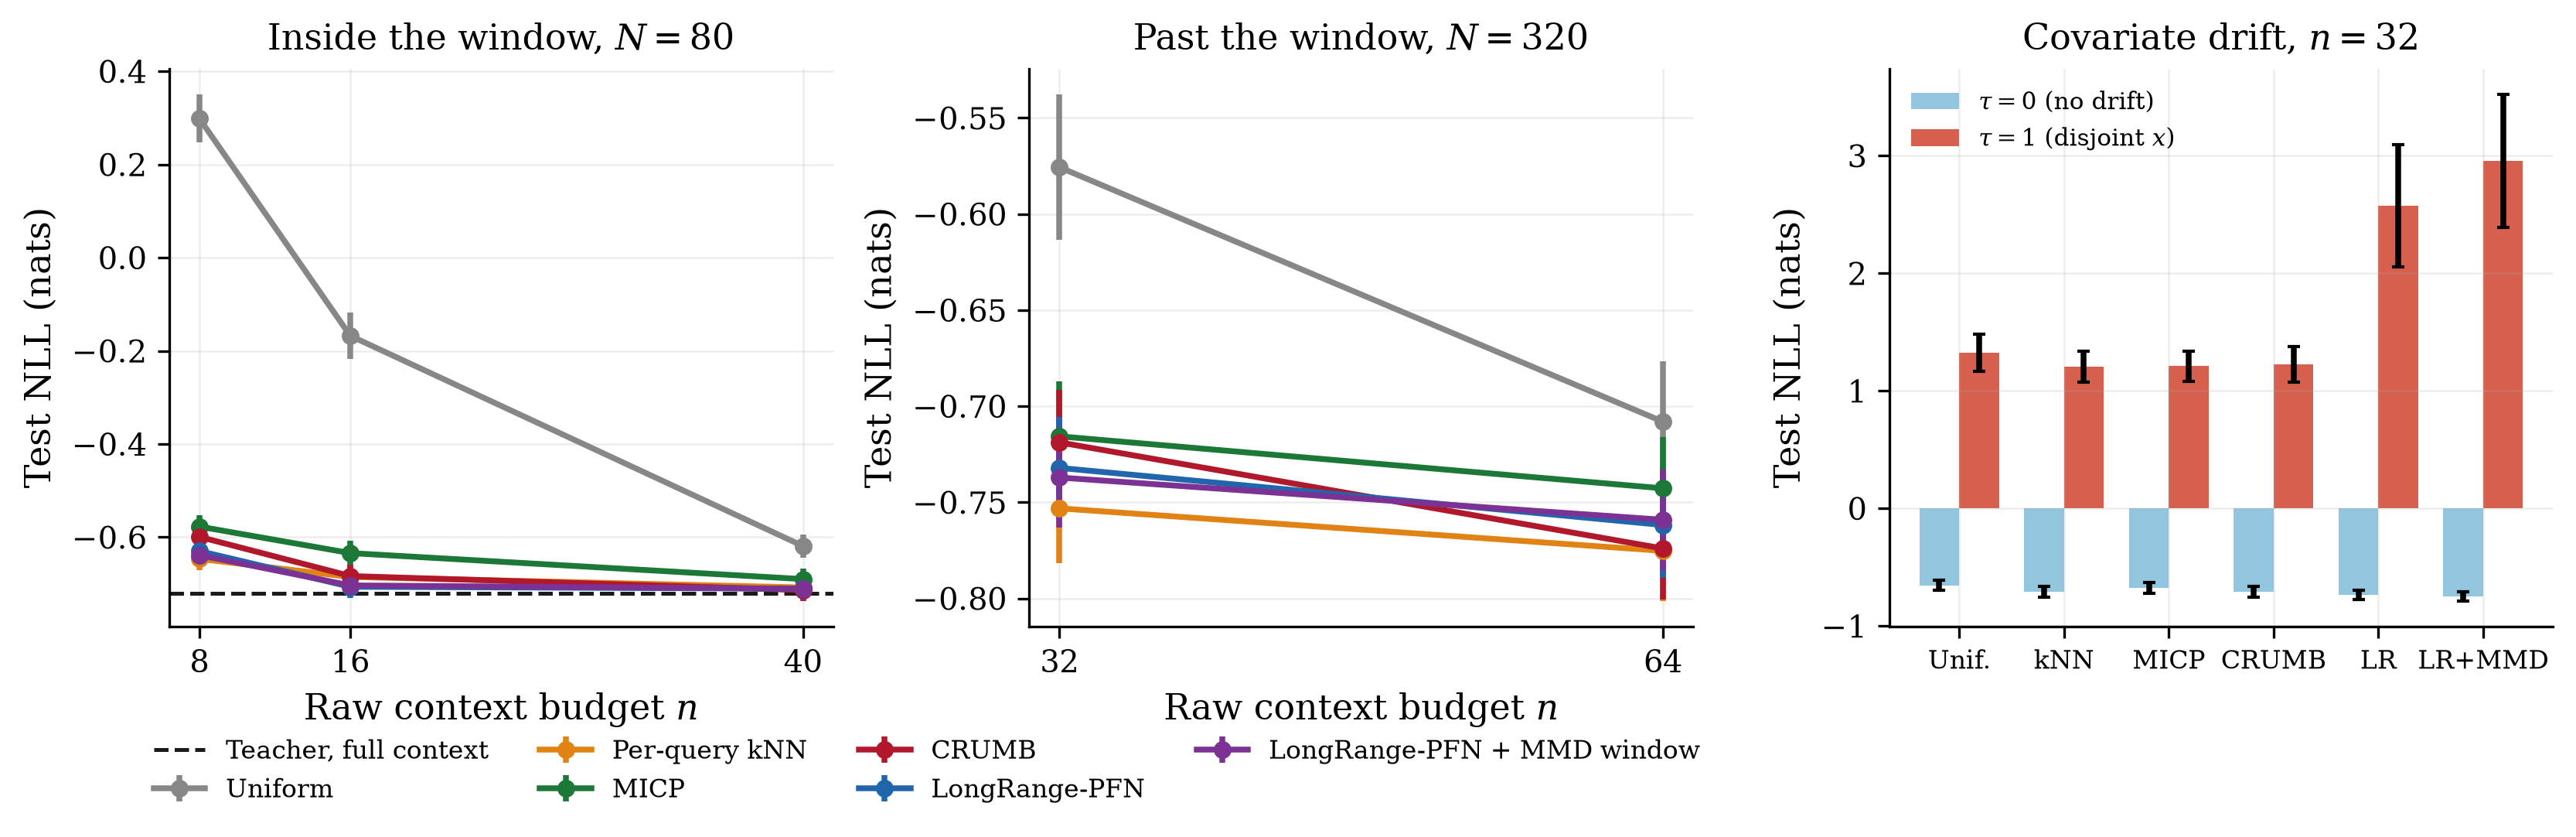
\includegraphics[width=0.95\textwidth]{../results/context_selection.png}
  \end{center}
\end{frame}

\begin{frame}{Where the method fits}
  \begin{columns}[T]
    \begin{column}{0.48\textwidth}
      \begin{block}{Latent summary}
        \begin{itemize}
          \item Moderate budget, test region matching the pool.
          \item Reusable \(O(k)\) state; raw points can be discarded.
          \item Every prefix \(z_t\) is already usable mid-stream.
        \end{itemize}
      \end{block}
    \end{column}
    \begin{column}{0.48\textwidth}
      \begin{block}{Test-time selectors}
        \begin{itemize}
          \item Tiny budget, or a pool far past the window.
          \item Disjoint covariate shift: the summary was trained on exchangeable data.
          \item CRUMB needs the test batch and carries no state across batches.
        \end{itemize}
      \end{block}
    \end{column}
  \end{columns}
  \vspace{0.8em}
  \footnotesize Multi-chunk cost is not a selection artifact: after fine-tuning with \(T>1\) in validation,
  KL still rises from \(0.019\) (\(T=1\)) to \(0.283\) (\(T=5\)).
\end{frame}

\begin{frame}{What remains}
  \begin{columns}[T]
    \begin{column}{0.48\textwidth}
      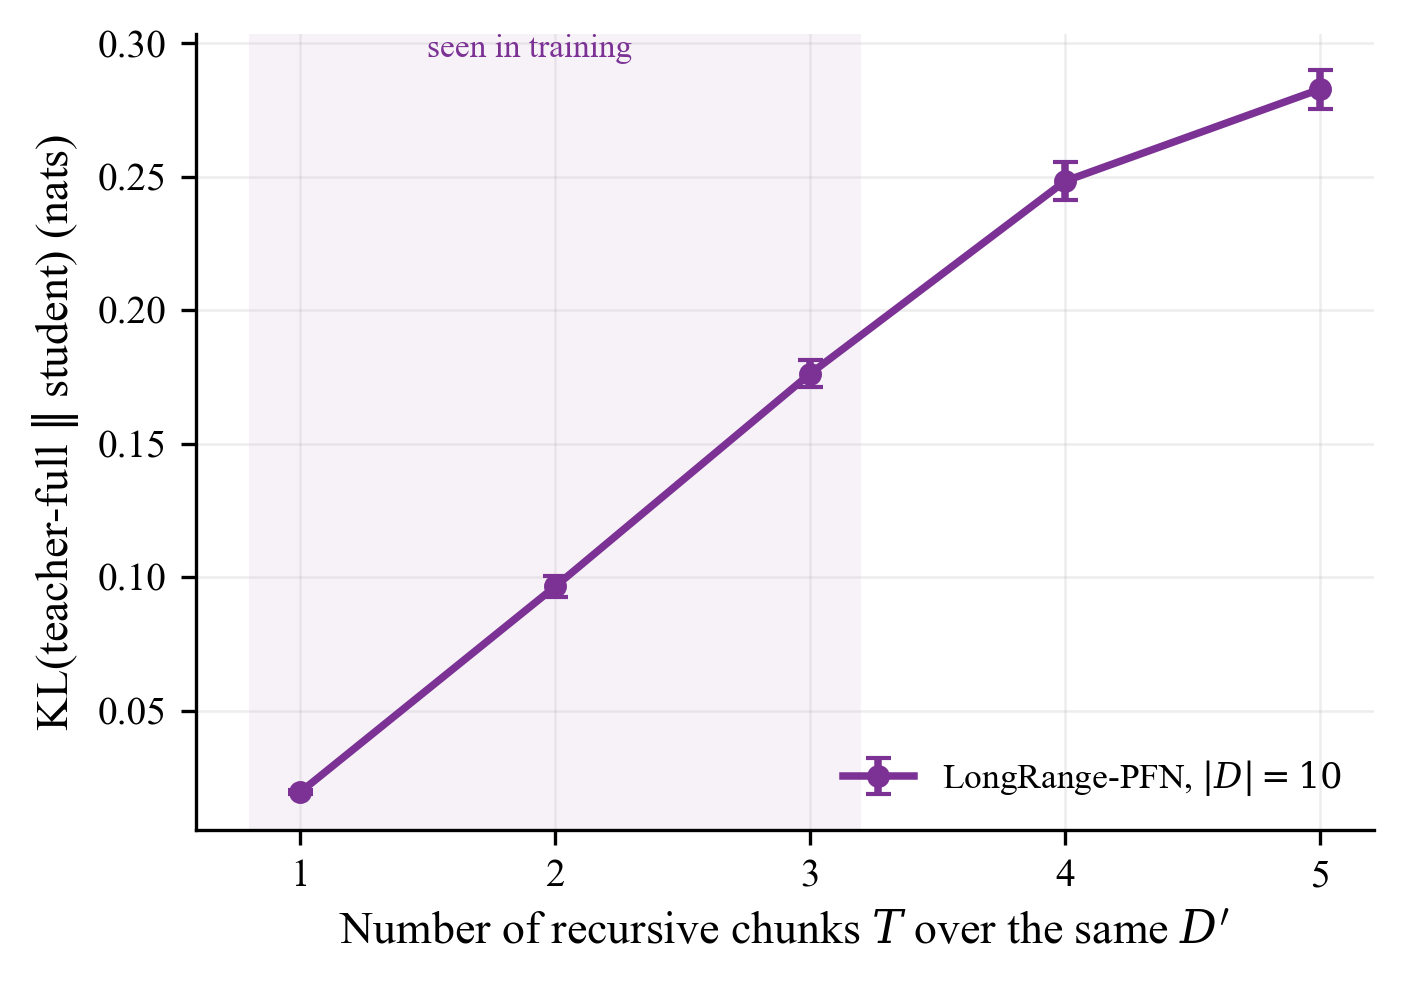
\includegraphics[width=\linewidth]{../results/chunks.png}
    \end{column}
    \begin{column}{0.48\textwidth}
      \begin{itemize}
        \item \textbf{Error that accumulates in \(T\).}
          Each \(\rep_\phi\) loses a little.
          Next: train with larger \(T\), or regularize associativity.
        \item \textbf{Proof of concept.}
          1D GP, small teacher. Next: intractable prior and a TabPFN-scale teacher.
        \item \textbf{Bottleneck and shift.}
          \(k=16\) is finite; under \(\tau=1\) the summary loses to local retrieval.
          Next: query-aware summary \(z(x)\).
      \end{itemize}
    \end{column}
  \end{columns}
\end{frame}

\begin{frame}
  \begin{center}
    {\Large\bfseries Bayesian evidence beyond the window,\\[0.25em] at constant state}
    \vspace{1.2em}

    Information from \(\Dfar\) reaches the predictor through \(z\):
    NLL crosses the Proposition~1 bound.\\[0.5em]
    The same state goes past a window of 80 and beats recency out to 320
    when the test region matches the pool.

    \vspace{1.8em}
    {\large Thank you. Questions.}
  \end{center}
\end{frame}

\end{document}
